\section{Introduction}

% Rise and Strengths of Multi-Agent LLMs
Inspired by Social Choice Theory \citep{Endriss17}, recent research considers the use of multiple large language models (LLMs) to solve complex reasoning tasks and mitigate the limitations of single models, such as lacking modularity and answer diversity \citep{YinSCG23a, ChenSB24a, SunYLW24}.
Agents, embedded with varying expertise, memory, planning, and tool use \citep{ChenSB24a, SunYLW24, ZhuangYWS23a, BakerKMW20a}, can emulate human interaction to solve problems \citep{GuoCWC24a, Becker24}.
Recent work highlights the strengths of multi-agent debate (MAD) in reasoning and creativity \citep{ZhaoHXL23a, XuYLW23a, SuzgunK24a}.
MAD also scales test-time compute to solve challenging tasks similar to reasoning models, such as OpenAI o4 \citep{OpenAIo4} and DeepSeek R1 \citep{deepseekai2025deepseekr1incentivizingreasoningcapability}, which can be more effective than scaling training compute or data \citep{SnellLXK24a}.
% These advancements have led to an increasing number of publications in the field.
%Multiple agents can be equipped with varying expertise or preferences, enhancing the discussions and the system's response over a single LLM \citep{ChenSB24, SunYLW24}.
%Under a fixed communication scheme that defines turn-taking, agents can be prompted to discuss potential solutions to a problem \citep{YinSCG23a}. 
%A decision-making mechanism checks for an agreement between the agents, producing a final output that aims to be superior to a single model.
%In general, a multi-agent LLM is a concept that considers agents, discussions, and decision-making for conversational problem-solving. 

\begin{figure}[t]
    \centering
    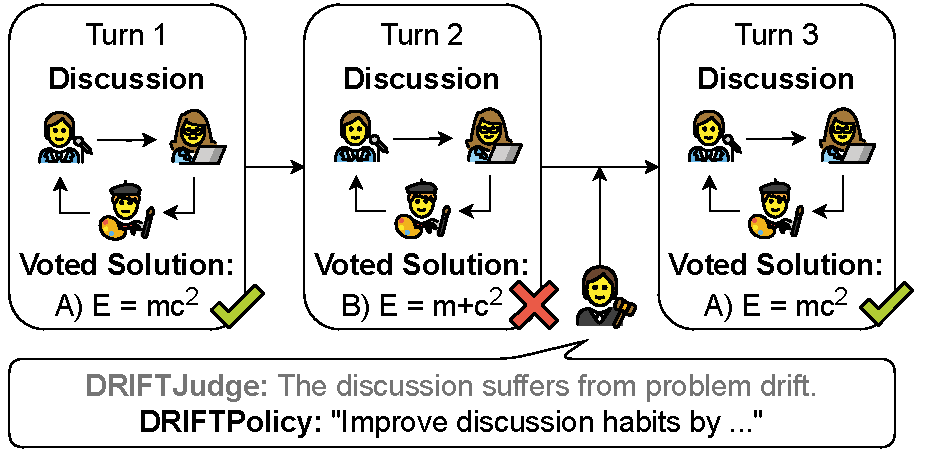
\includegraphics[width=0.99\linewidth]{figures/other_charts/problem_drift.pdf}
    \caption{Problem drift in MAD. \judge\ detects problem drift at test-time. \policy\ provides on-demand feedback about the conversation.}
    \label{fig:problem_drift}
\end{figure}

% Problems of Multi-Agent Research => Whats the gap?
However, the increasing complexity of MAD can promote errors and undesired behaviors (e.g., propagating hallucinations) \citep{GuoCWC24a}.
Problems originating from debate comprise agent orchestration \citep{WangWST24, ShahW24}, diminished planning capabilities \citep{ValmeekamMK23a}, and ineffective criticism generated by the LLM \citep{StechlyMK23a}.
Still, it is largely unknown what causes MAD to fail and why it happens.
It remains uncertain how MAD can avoid issues like ineffective criticism, which is crucial for high-quality debate and reliable results.
Few mitigation methods have been proposed for the few errors identified by related work.
% This is relevant as using LLMs as agents, their scale and interaction have gained significant attention \citep{WangMFZ24a}.
% Thus, we need to quantify how reliable agents are in such scenarios to deploy multi-agent systems efficiently.
%To quantify the limitations of agentic problem-solving, we provide an initial investigation, paving the way for subsequent advancements in the field.

% Other studies identify the limitations of multi-agent systems (e.g., agent orchestration) \citep{WangWST24, ShahW24a}, illustrating the prevailing uncertainty among scholars regarding the effectiveness of LLMs in a multi-agent setup.
% Meanwhile, the increasing complexity of these systems often promotes errors or unwanted behaviors \citep{GuoCWC24}.
% We lack a thorough understanding of the scenarios in which multi-agent systems fail.
% Specifically, whether and how continuous multi-agent interaction could affect performance is still under-explored.
% This is relevant as using LLMs as agents, their scale and interaction have gained significant attention as a promising direction for artificial intelligence \citep{WangMFZ24a}.
% Thus, we need to quantify how reliable agents are in such scenarios to deploy multi-agent systems efficiently and safely.
% To quantify the limitations of agentic problem-solving, we provide an initial investigation, paving the way for subsequent advancements in the field.

% Where do we step in? What do we do? 
This paper systematically analyzes errors that lead to performance degradation in MAD.
Through automated methods and a human evaluation, we observe that multi-agent systems can collapse in long discussions.
In some debates, agents' communication tends to deteriorate over time, drifting to a point where they can not recover and address the original task goal.
We refer to this phenomenon as \textbf{problem drift} and investigate its underlying causes and effects.
To identify problem drift post-hoc in MAD, we propose \metric, a simple yet effective metric that measures the quality of the ongoing discussion.
%We study a total of ten tasks for problem drift: three generative (i.e., XSum \citep{NarayanCL18b}, ETPC \citep{KovatchevMS18b}, WMT19 \citep{WikimediaFoundation19}), three reasoning (i.e., StrategyQA \citep{GevaKSK21}, WinoGrande \citep{SakaguchiBBC19}, AQUA-RAT \citep{LingYDB17a}), three knowledge tasks (i.e., ETHICS \citep{HendrycksBBC23}, MMLU-Pro \citep{WangMZN24}, GPQA \citep{ReinHSP23a}), and one instruction following task (i.e., IFEval \citep{ZhouLMB23}).
% We examine how multi-agent discussions unfold and investigate their performance convergence, i.e., \textit{problem focus}, by testing ten datasets from generative, knowledge, reasoning, and instruction-following tasks.
% We find that while multi-agent discussions can occasionally improve the performance of the final solution, they often fail to debate effectively for longer periods.
% Our investigation shows that conversations can suffer from incremental performance collapse, called \textit{problem drift}.
% What are the findings? What is the impact of these findings.
%We test ten tasks (i.e., MMLU, ....) for the identified issue.
Our results suggest that problem drift occurs across all tested tasks, being most prevalent in generative tasks (76\%-89\% of samples), followed by instruction-following tasks (21\% of samples).
The majority of observed drifts do not recover.
Once a discussion drifts away, agents often do not reach the correct solution for a given task, except in 9\% of the translation and 45\% of the ethical question-answering examples. %here
%The good news is that problem drift is not necessarily irrecoverable.
% To identify problem drift at test-time, we propose \judge, based on LLM-as-a-judge \citep{ZhengCSZ23}, and \policy, a new method based on a policy feedback agent \citep{FuPKL23b} that advises participating agents to improve the debate (\Cref{fig:problem_drift}).
To identify and mitigate problem drift at test-time, we propose \judge\ and \policy.
While \judge\ identifies problem drift acting as an LLM-as-a-judge \citep{ZhengCSZ23}, \policy\ introduces a policy feedback agent \citep{FuPKL23b} that advises participating agents to improve the debate.
\Cref{fig:problem_drift} shows the dynamics between \judge\ and \policy\ during MAD.
We show that \policy\ can reduce the number of drifting discussions by 31\%, improving task accuracy by up to 3.6\% for weaker model agents.

By asking eight human experts, we identify eight reasons why problem drift occurs in MAD and categorize them into temporal error types (e.g., lack of progress) and local error types (e.g., task non-compliance).
Agent discussions are especially prone to a lack of progress (35\% of drifting samples) that can lead agents to overanalyze problems and give low-quality feedback.
Our work can be seen as a systematic analysis of MAD, showing the inherent limitations of prolonged agent interaction.
%The good news is that problem drift is not necessarily irrecoverable.
%To identify problem drift at test-time, we propose \judge, based on LLM-as-a-judge \citep{ZhengCSZ23}, and \policy, a new method based on a policy feedback agent \citep{FuPKL23b} that advises participating agents to improve the debate (\Cref{fig:problem_drift}).
%We show that \policy\ can reduce the number of drifting discussions by 31\%.
%Our work can be seen as a window into the heart of MAD, showing the inherent limitations of long agent interaction.
%By investigating the intrinsic characteristics of the debate, we pave the way for subsequent advancements in the field of multi-agent LLMs for problem-solving.
We release the code and data publicly\footnote{\mbox{\url{https://github.com/jonas-becker/problem-drift}}}.
% The main contributions of this work are:
% \begin{itemize}
%     \item We identify problem drift as a cause for performance degradation in multi-agent debate.
%     \item We quantify the prevalence and recoverability of problem drift. 
%     \item We explore the most common error types related to problem drift according to humans.
%     \item We propose \judge\ and \policy\ to detect and mitigate problem drift.
% \end{itemize}

% Research Questions
%We explore the following research questions:

% \begin{enumerate}
%     \item \textbf{Can prolonged multi-agent discussion harm task performance?}
%     \begin{enumerate}
%         \item How do multi-agent systems perform across tasks? What are the characteristics of resulting discussions?
%         \item How does the length of multi-agent discussion impact task performance?
%         \item How strong is the identified problem drift and does it depend on the task?
%         \item Can discussions recover from problem drift?
%     \end{enumerate}
    
%     \item \textbf{How can we address problem drift in an ongoing discussion?}
%     \begin{enumerate}
%         \item What are the reasons for problem drift as judged by human experts? %Are there common problems occurring in the same tasks or across tasks?
%         \item Can we mitigate problem drift when we know that it occurs?
%         \item Can we identify problem drift at test-time when the gold labels are unknown?
%     \end{enumerate}
% \end{enumerate}

% What are the main findings of the paper?
% \noindent
% The main finding of the paper is that while multi-agent discussions can occasionally improve the performance of the final solution, they often fail to discuss effectively for longer durations.
% Our investigation shows that conversations can suffer from incremental performance collapse.
% We identify and highlight several reasons for this problem drift.
% Concretely, LLMs have the tendency to prefer shorter responses by other agents, distorting the decision-making process.
% Generative tasks suffer from minor incremental changes to the solution. 
% Problem drift on multiple-choice tasks is stronger but also easier to recover from.
% By systematic extraction and asking eight human experts in natural language processing, we discover eight temporal and local error types that are related to problem drift.
% Discussions are especially prone to a lack of progress that can lead to agents overanalyzing the problem and failing to give high-quality feedback.
% Using our discovered error types that are relevant to problem drift, we employ an LLM-as-a-judge \citep{ZhengCSZ23} to effectively identify problem drift at test-time.
% We introduce a policy feedback agent \citep{FuPKL23} to the conversation as an effective mitigation strategy with reasonable compute requirements.